
% Features:
%  � Proper page sizes as required by university guide for students:
%      � proper font sizes as well as linespacings
%      � proper size of margins
%  � Generic title page:
%      � \gentitle
%  � Generic abstract page(s):
%      � \begin{itabstract}{Keywords}
%          abstract text
%        \end{itabstract}
%      � \begin{ittiivis}...\end{ittiivis} provides finnish version
%         � ittiivis defaults to finnish so no need to issue 
%           \selectlanguage{finnish}
%      � total number of pages as well as total number of pages in appendices
%        are automagically handled
%  � Entry environment:
%      � \begin{entry}[widest label]
%          \item[1st label text] ...
%          \item[2nd label text] ...
%        \end{entry}
%      � the actual items are aligned to suit the widest label, which is
%        given as an argument to the environment
%  � Use of specific latex packages to ease in formatting the thesis:
%      � format table of contents to have bibliography shown as references
%        as well as other fixes           (tocbibind)
%      � enhanced verbatim handling       (sverb)
%      � source code inclusion            (listings)
%      � handling of headers and footers  (fancyhdr)
%
%      � consultation of the manuals of these packages is strongly
%        encouraged 
%
% Assumptions:
%  � itpackage.sty file is available 
%  � each chapter is as a separate file which is read in with e.g. \input
%   
% Miscellaneous:
%  � comments are welcome
%  � should a required package be missing see http://www.ctan.org/ 
%  � http://www.ctan.org/tex-archive/info/lshort/english/lshort.pdf
%
%%%%%%%%%%%%%%%%%%%%%%%%%%%%%%%%%%%%%%%%%%%%%%%%%%%%%%%%%%%%%%%%%%%%%%%%%%%

%%%%%%%%%%%%%%%%%%%%%%%%%%%%%%%%%%%%%%%%%%%%%%%%%%%%%%%%%%%%%%%%%%%%%%%%%%%
%
% load all required packages
%
%%%%%%%%%%%%%%%%%%%%%%%%%%%%%%%%%%%%%%%%%%%%%%%%%%%%%%%%%%%%%%%%%%%%%%%%%%%

\documentclass[a4paper,12pt]{report}
\usepackage{amssymb,amsthm,amsmath}
\usepackage[english,finnish]{babel}
\usepackage[latin1]{inputenc}
\usepackage{ifpdf}
\usepackage{graphicx}
\usepackage[nottoc]{tocbibind}
\settocbibname{References}
\usepackage{sverb}
\usepackage{listings}
\usepackage{fancyhdr}
\usepackage{itpackage}
\usepackage{cite}
\usepackage{placeins}
\usepackage{pifont}
\usepackage{array}
\usepackage{balance}
\usepackage{refstyle}
\usepackage{pgfplots}
\usepackage{bchart}
\setlength{\parindent}{15pt}
\newcolumntype{C}[1]{>{\centering\let\newline\\\arraybackslash\hspace{0pt}}m{#1}}
\usepackage{caption}
\usepackage{amsfonts}
\usepackage{color,soul}


% uncomment the following snippet to get rid of Luku/Chapter text at the
% beginning of each Chapter... 
%\makeatletter
%\renewcommand{\@chapapp}{\relax}
%\renewcommand{\@makechapterhead}[1]{%
%  \vspace*{50\p@}%
%  {\parindent \z@ \raggedright \normalfont
%    \ifnum \c@secnumdepth >\m@ne
%        \huge\bfseries \@chapapp\space \thechapter\space\space
%    \fi
%    \interlinepenalty\@M
%    \Huge \bfseries #1\par\nobreak
%    \vskip 40\p@
%  }}
%\makeatother

%%%%%%%%%%%%%%%%%%%%%%%%%%%%%%%%%%%%%%%%%%%%%%%%%%%%%%%%%%%%%%%%%%%%%%%%%%%
%
% main document starts here
%
%%%%%%%%%%%%%%%%%%%%%%%%%%%%%%%%%%%%%%%%%%%%%%%%%%%%%%%%%%%%%%%%%%%%%%%%%%%
\begin{document}

% select language here by removing comment from one of the two rows below
% \selectlanguage{finnish}\fintrue
\selectlanguage{english}\def\enclname{Appendices}\finfalse

%%% fill in your information below
\workinfo{Mohammad Reza Memarian}
{BotCloud Detection System}
{Ville Lepp�nen}
{Mauro conti}
{2015}
{August}

% set the type of your thesis (Diplomity�, TkK -tutkielma, etc.) and
% laboratory or field of study below
\worktype{Master thesis}{Ty�n tyyppi} 
\deptinfo{Information Security and Cryptography}


% generate the title page 
\gentitle

% generate tiivistelma 

% if your thesis is in english then this is also required (is it???)
\begin{itabstract}{Botcloud; cloud computing; misuse detection; virtual machine introspection. }
Leveraging cloud services, companies and organizations can significantly improve their efficiency, as well as building novel business opportunities. A significant research effort has been put in protecting cloud tenants against external attacks. However, attacks that are originated from elastic, on-demand and legitimate cloud resources should still be considered seriously. The cloud-based botnet or botcloud is one of the prevalent cases of cloud resource misuses. Unfortunately, some of the cloud's essential characteristics enable criminals to form reliable and low cost botclouds in a short time. In this paper, we present a system that helps to detect distributed infected Virtual Machines (VMs) acting as elements of botclouds. Based on a set of botnet related system level symptoms, our system groups VMs. Grouping VMs helps to separate infected VMs from others and narrows down the target group under inspection. Our system takes advantages of Virtual Machine Introspection (VMI) and data mining techniques.
\end{itabstract}


% empty pagestyle for table of contents etc. 
%
% the redefinition of plain style works also for 1st pages of chapters,
% which is the default in report class. Just state \thispagestyle{empty}
% after \chapter{something} if you want empty style for the 1st pages. 
%
\pagestyle{empty}
\fancypagestyle{plain}{
  \fancyhf{}
  \renewcommand{\headrulewidth}{0 pt}
}

% roman numbering for table of contents etc.
\pagenumbering{roman}

% insert table of contents, list of figures, list of tables
%
% setting the counter to zero effectively removes the page number from
% the toc, lof etc. entries in the toc since there is no roman numeral
% for zero ;-) (if you want them without numbering)
%
%\setcounter{page}{0}
\tableofcontents
\clearpage
%\setcounter{page}{0}
\listoffigures 
\clearpage
%\setcounter{page}{0}
\listoftables

% possibly insert 'list of acronyms'
%
%   � create a chapter called List Of Acronyms (or whatever), which
%     should contain all your acronym definitions, e.g. 
%     \chapter{List Of Acronyms} 
%   � the secnumdepth trickery is needed because acronyms are as a
%     standard chapter and we are faking '\listofacronyms'
%
%	\setcounter{secnumdepth}{-1}
%\input{your acronym chapter's file name}
%\setcounter{secnumdepth}{2}


% setup page numbering, page counter, etc.
\startpages

%%%%%%%%%%%%%%%%%%%%%%%%%%%%%%%%%%%%%%%%%%%%%%%%%%%%%%%%%%%%%%%%%%%%%%%%%%%
%
% hi ho hi ho it's off to work we go....
%
% from now on you're on your own -- good luck!
%
% that is to say that the actual thesis should come here 
%
%%%%%%%%%%%%%%%%%%%%%%%%%%%%%%%%%%%%%%%%%%%%%%%%%%%%%%%%%%%%%%%%%%%%%%%%%%%
%%%%%%%%%%%%%%%%%%%%%%%%%%%%%%%%%%%%%%%%%%%%%%%%%%%%%%%%%%%%%%%%%%%%%%%%%%%
%%%%%%%%%%%%%%%%%%%%%%%%%%%%%%%%%%%%%%%%%%%%%%%%%%%%%%%%%%%%%%%%%%%%%%%%%%%
%%%%%%%%%%%%%%%%%%%%%%%%%%%%%%%%%%%%%%%%%%%%%%%%%%%%%%%%%%%%%%%%%%%%%%%%%%%
%%%%%%%%%%%%%%%%%%%%%%%%%%%%%%%%%%%%%%%%%%%%%%%%%%%%%%%%%%%%%%%%%%%%%%%%%%%
%%%%%%%%%%%%%%%%%%%%%%%%%%%%%%%%%%%%%%%%%%%%%%%%%%%%%%%%%%%%%%%%%%%%%%%%%%%
%%%%%%%%%%%%%%%%%%%%%%%%%%%%%%%%%%%%%%%%%%%%%%%%%%%%%%%%%%%%%%%%%%%%%%%%%%%
%%%%%%%%%%%%%%%%%%%%%%%%%%%%%%%%%%%%%%%%%%%%%%%%%%%%%%%%%%%%%%%%%%%%%%%%%%%

%\input{file name of chapter xxx}
%\input{file name of chapter yyy}
%\input{file name of chapter zzz}
%\input{and so on...}
\chapter{Introduction}
Cloud computing is a powerful technology for delivering on-demand hosted services in a multi-tenant environment. It enables consumers to have access to a vast amount of computing resources at any desired time. Cloud computing provides suitable infrastructure, for both honest and malicious purposes. On demand self service resources and rapid elasticity are characteristics of cloud computing that create opportunities for cyber criminals to get advantage of cloud resources. As discussed in \cite{ref1}, abuse of cloud services is a prevalent threat to cloud computing. This matter raises the importance of detection and prevention of abuse uses of cloud services for Cloud Service Provider (CSP). A distinctive example of these kinds of anomalistic usages of cloud services is formation of botnet in the cloud.\\

Botnet is a group of infected computer systems that enables a controller to have control over the group. Examples of botnet functions are: DDoS attack, spamming, search engine optimization poisoning, pay-per-click fraud, financial fraud, bitcoin mining and information stealing \cite{ref22}, \cite{ref34}. Botmasters specifically benefit from the cloud's provided infrastructure as cloud computing offers them various possibilities to conduct their desired attacks. In cloud computing, fairly cheap, scalable and reliable resources are always ready for use. So attackers have ready-to-use infrastructure for their malicious activities. Forming a reliable botclould is an easy and low cost procedure while anonymity of criminals can be preserved \cite{ref42}. \\

Botnets are moving toward being more elusive which are able to escape detection. Botmasters integrate multiple backup forms of command and control to hide commanding servers. Particularly, DDoS attacks as a consequence of botnets tend to change their attack vectors during a single attack. As described in \cite{ref14}, botnets are becoming more resilient and responding faster to countermeasures, while getting larger in attack volume and frequency of occurrence\cite{ref16}. \\

There are various issues that pave the path for criminals to form a botcloud much easier compared to forming a botnet in conventional environments. Some of these issues are: trendiness of large scale diverse attacks \cite{ref36}, cloud specific vulnerabilities \cite{ref9} and some of cloud essential characteristics \cite{ref40}. Specific features of cloud computing such as image sharing and interest for homogeneity among cloud systems can further ease the formation of botclouds.   \\ 

Main botnet detection methods are: honeypot and intrusion detection system (IDS). Using honeypot and applying intrusion detection system on each machine in the cloud are not feasible solutions \cite{ref42} \cite{ref38}. On the other hand, distributed and specific structure of cloud computing requires detection solutions to meet various cloud specific considerations. In order to detect cloud resource misuses, researchers proposed cloud specific detection systems while mostly overlooking prevention capability in their designed systems. Unfortunately, the solutions for detection of botnets in the cloud are not mature yet; in fact attacks using cloud resources are on rise.\\

In response to challenges above, a BotCloud Detection System (BCDS) needs to: 1) have a broad view over all nodes in the cloud in a cloud-wide manner; 2) be based on cloud core technologies; 3) be reliable for large cloud environments while being effective. \\

\textbf{Contribution.}
In this document we propose a botcloud detection system that tackles the problem of detecting when infected VMs in a cloud form botclouds. Our system adopts new approaches toward data gathering, information correlation and decision making steps. We propose the main correlation module to be placed in an outer level of cloud platform which is the cloud controller. This helps the system to be more practical and have a wider view over the cloud nodes. In data gathering phase, our approach takes advantage of virtualization as one of the cloud core technologies \cite{ref9}. Our system has various detectors in each host that makes the design more reliable. Our result shows that based on the selected attributes, infected VMs that are potential security threats, can be separated from other VMs. \\

\textbf{Organization.}
The rest of this document is organized as follows. Chapter 2 gives background information. Chapter 3 explains existing approaches for botcloud detection and malware analysis using VMI in the cloud. In Chapter 4 we introduce our novel design for detection of infected systems which can be elements of botclouds, while in Chapter 5 we discuss implementation details. In Chapter 6 we discuss and evaluate our results, and in Chapter 7 we explain our conclusion and future research direction.\\

\chapter{PRELIMINARY INFORMATION }
In this Chapter, we give some preliminary information to make understanding of rest of this document smoother. In particular, we explain preliminary knowledge about cloud computing (Section 2.1), virtualization (Section 2.2), botcloud (Section 2.3), VMM (Section 2.4) and VMI (Section 2.5). 

\section{Cloud Computing}
Cloud computing is an advanced computing model which enables access to a pool of shared, configurable computing resources. Cloud computing provides various opportunities specifically for small to medium level enterprises (SMEs). In other word, cloud computing offers hosted services over the internet to the consumers. Depending on consumer needs, various costs can be saved by getting benefits from cloud computing. \\

Cloud computing enables service providers to offer variety of cloud based services to the customers. The cloud services vary from storage, networking and computation to applications. For example, a consumer can save his private data on the cloud storage services. In this way the consumer does not invest any more in storage devices. Also, the responsibility of providing high availability services will be offloaded to the service provider. Another example is a consumer which needs high computing resources only in some specific times. Instead of investing in computing resources, he can consume cloud resources whenever he needs the service.  \\ 

Cloud computing enables consumers to use computing resources as utilities. So consumers pay only for the service that they used. There are different ways to calculate consumer's usages. Basically calculation of usage varies from provider to provider and depends on used service. In other word, consumers pay for the metered service and pay only for the exact usage. By using the word consumer, we refer to individual users in addition to enterprises. \\

Cloud computing has various advantages and benefits for consumers. Some of the advantages are in the following:\\

\begin{itemize}
\item Implementation speed reduces as customers do not need to invest in time for research, training and implementation matters related to new systems.
\item Consumers can rapidly scale their service to meet their needs. This point addresses consumer's needs that arise based on unpredictable events.
\item Consumers can have access to their anywhere using a standard internet connection. So basically access anywhere model can be reached. 
\item Consumers can have access to their anywhere using a standard internet connection. So basically access anywhere model can be reached. 
\item Consumers offload responsibilities such as software update, patches, licences and hardware maintenance to the service provider. So IT staff of companies can have more productivities by not getting engaged with the mentioned concerns.
\end{itemize}

Cloud computing has some powerful and specific characteristics which make the cloud very powerful. Based on \cite{ref40}, cloud computing has five essential characteristics. These characteristics are: 
\begin{itemize}
\item On-demand self-service 
\item Broad network access
\item Resource pooling
\item Rapid elasticity
\item Measured services
\end{itemize}
 
All mentioned characteristics are vital and specific to the cloud computing. Each of them has some benefits for the consumers. On-demand self-service allows consumers to provision resources as much as required. Broad network access means that cloud resources are available for access through several devices (Laptop, smart phones and etc.) and from various locations. Resource pooling refers to cloud service provider resources which are pooled. The resources serve various users in a multi-tenant environment. As addressed earlier, some of the cloud resources are storage, processing and network bandwidth. Rapid elasticity refers to the ability of consumer which can rapidly occupy and release the computing resources. Measured services refers to the fact that cloud services are measured based on some metrics. These metrics are either time or amount of usage or any other suitable metric. \\
 
From implementation point of view, there are four deployment models in addition to three service models for the cloud \cite{ref40}. We discuss deployment and service models in the following parts.  \\
 
\subsection{Deployment models}
\paragraph{Private cloud.}
Private cloud is a type  of cloud infrastructure that is operated for only one organization. This type of infrastructure can either be operated by the using enterprise itself or a third party. The private cloud infrastructure can be hosted either inside or outside the organization. In other word, an organization can request from a service provider for dedicated a infrastructure. So the specific consumer uses the dedicated infrastructure solely. This is the case that private cloud is operated by the third part outside of the company. However, companies can set up their own private cloud and operate it in the physical barriers of the company. So, private cloud model provide computing power to specific users by providing pool of physical resources. \\ 

The private cloud model is closer to conventional organization's networks than other deployment models. The private cloud deployment offer various kind of advantages. Consumers of private cloud architecture compared to other models (in particular public model) can benefit from advantages such as: higher security and privacy, cloud bursting, more efficiency and reliability. 

\paragraph{Public cloud.} 
Public cloud is referred to a kind of a cloud deployment model which is ready to use for all public consumers. Various consumers should use shared underlying infrastructure. there are variety of enterprises that offer public cloud services. Some of the most important ones are: amazon, rackspace and google. Basically the advantage of this deployment model is in multi-tenancy. Various consumers may use and share same resources. So service provider shares the cost among them. In addition to that, devices such as servers, run with more load. So servers resources do not get wasted as in the case of organizations. Normally in the organizations, servers and computing resources do not run with full load. \\

As shown in Figure 2.1, in public cloud deployment model various consumers use shared resources. Although multi-tenancy opens up opportunities, but it is a major threat toward security and privacy of users data.  \\

Public cloud deployment model offers some advantages to consumers compared to other deployment models. The benefits of public cloud deployment models are: ultimate scalability and reliability; location independence and utility model metering and payment. 


\begin{figure*}
\begin{center}
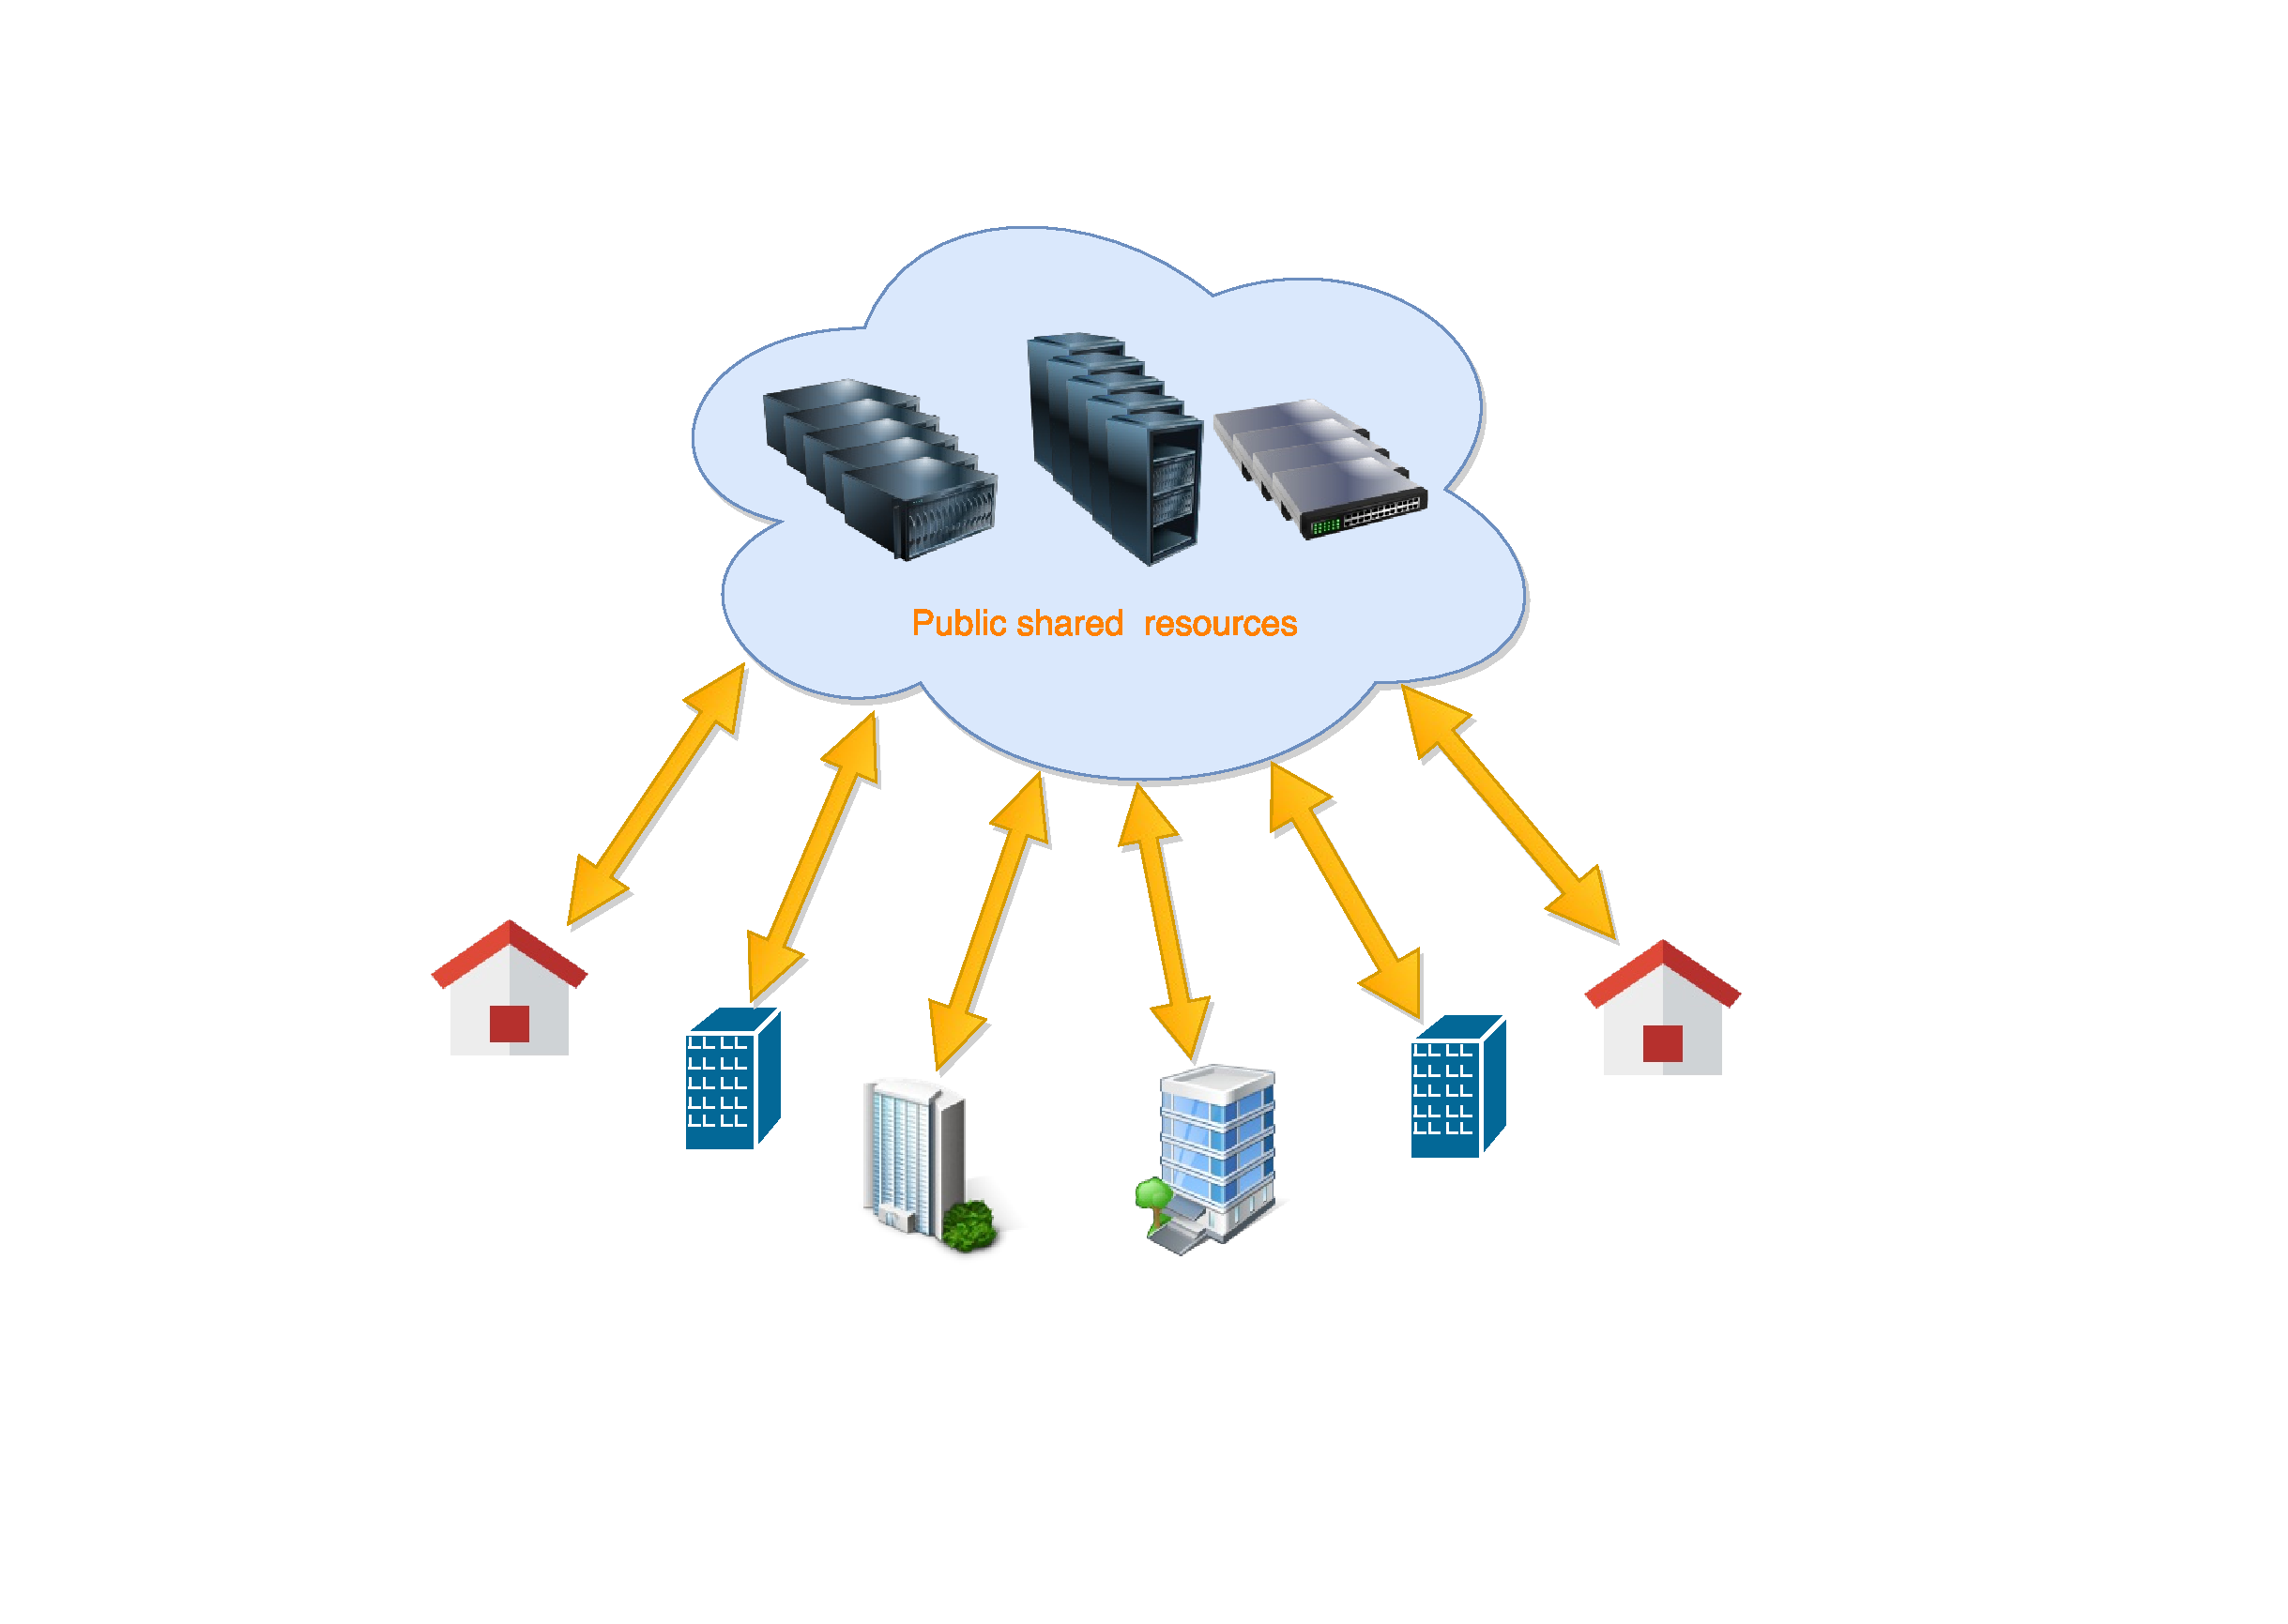
\includegraphics[scale=0.3]{publiccloud.pdf}
\caption{A high level public cloud architecture}
\end{center}
\end{figure*}

\paragraph{Hybrid cloud.}
Hybrid model is a kind of combination model between other deployment models (mostly public and private deployment models). Computing needs can move back and forth between public and private cloud of consumers. For example, an enterprise can have critical data and computation running on own private cloud while the less critical and private data and computation to take place on a reputable public cloud. Indeed, one of the advantages of private cloud deployment model which we addresses was cloud bursting. Cloud bursting has a high similarity with definition of hybrid cloud. Hybrid model benefits from characteristics of all other 3 deployment models while depending on various service providers. So there are not clear boundaries between service providers services in this model as private and public models. \\

As mentioned earlier, the core idea at back of the hybrid cloud deployment model is getting benefit of various deployment models. So a prevalent use case is when consumers use their own private cloud and in time of need, they consume the resources available in public or community cloud. 
 
\paragraph{Community Cloud.}
Community cloud is a type of cloud deployment model that several organizations with same concern, policy and need share a cloud infrastructure. As a result, costs are shared among all the consumers. Community cloud as other deployment models (in particular private model) can either be deployed and hosted internally or externally. Also community cloud consumers can either control and maintain the service by themself or a third party can handle maintenance. The third party can either be a CSP that offers cloud services to other enterprises too or it can be a company that maintains an specific community cloud. As depicted in Figure 2.2, organizations with same concern and policies may share same cloud resources.   

\begin{figure*}
\begin{center}
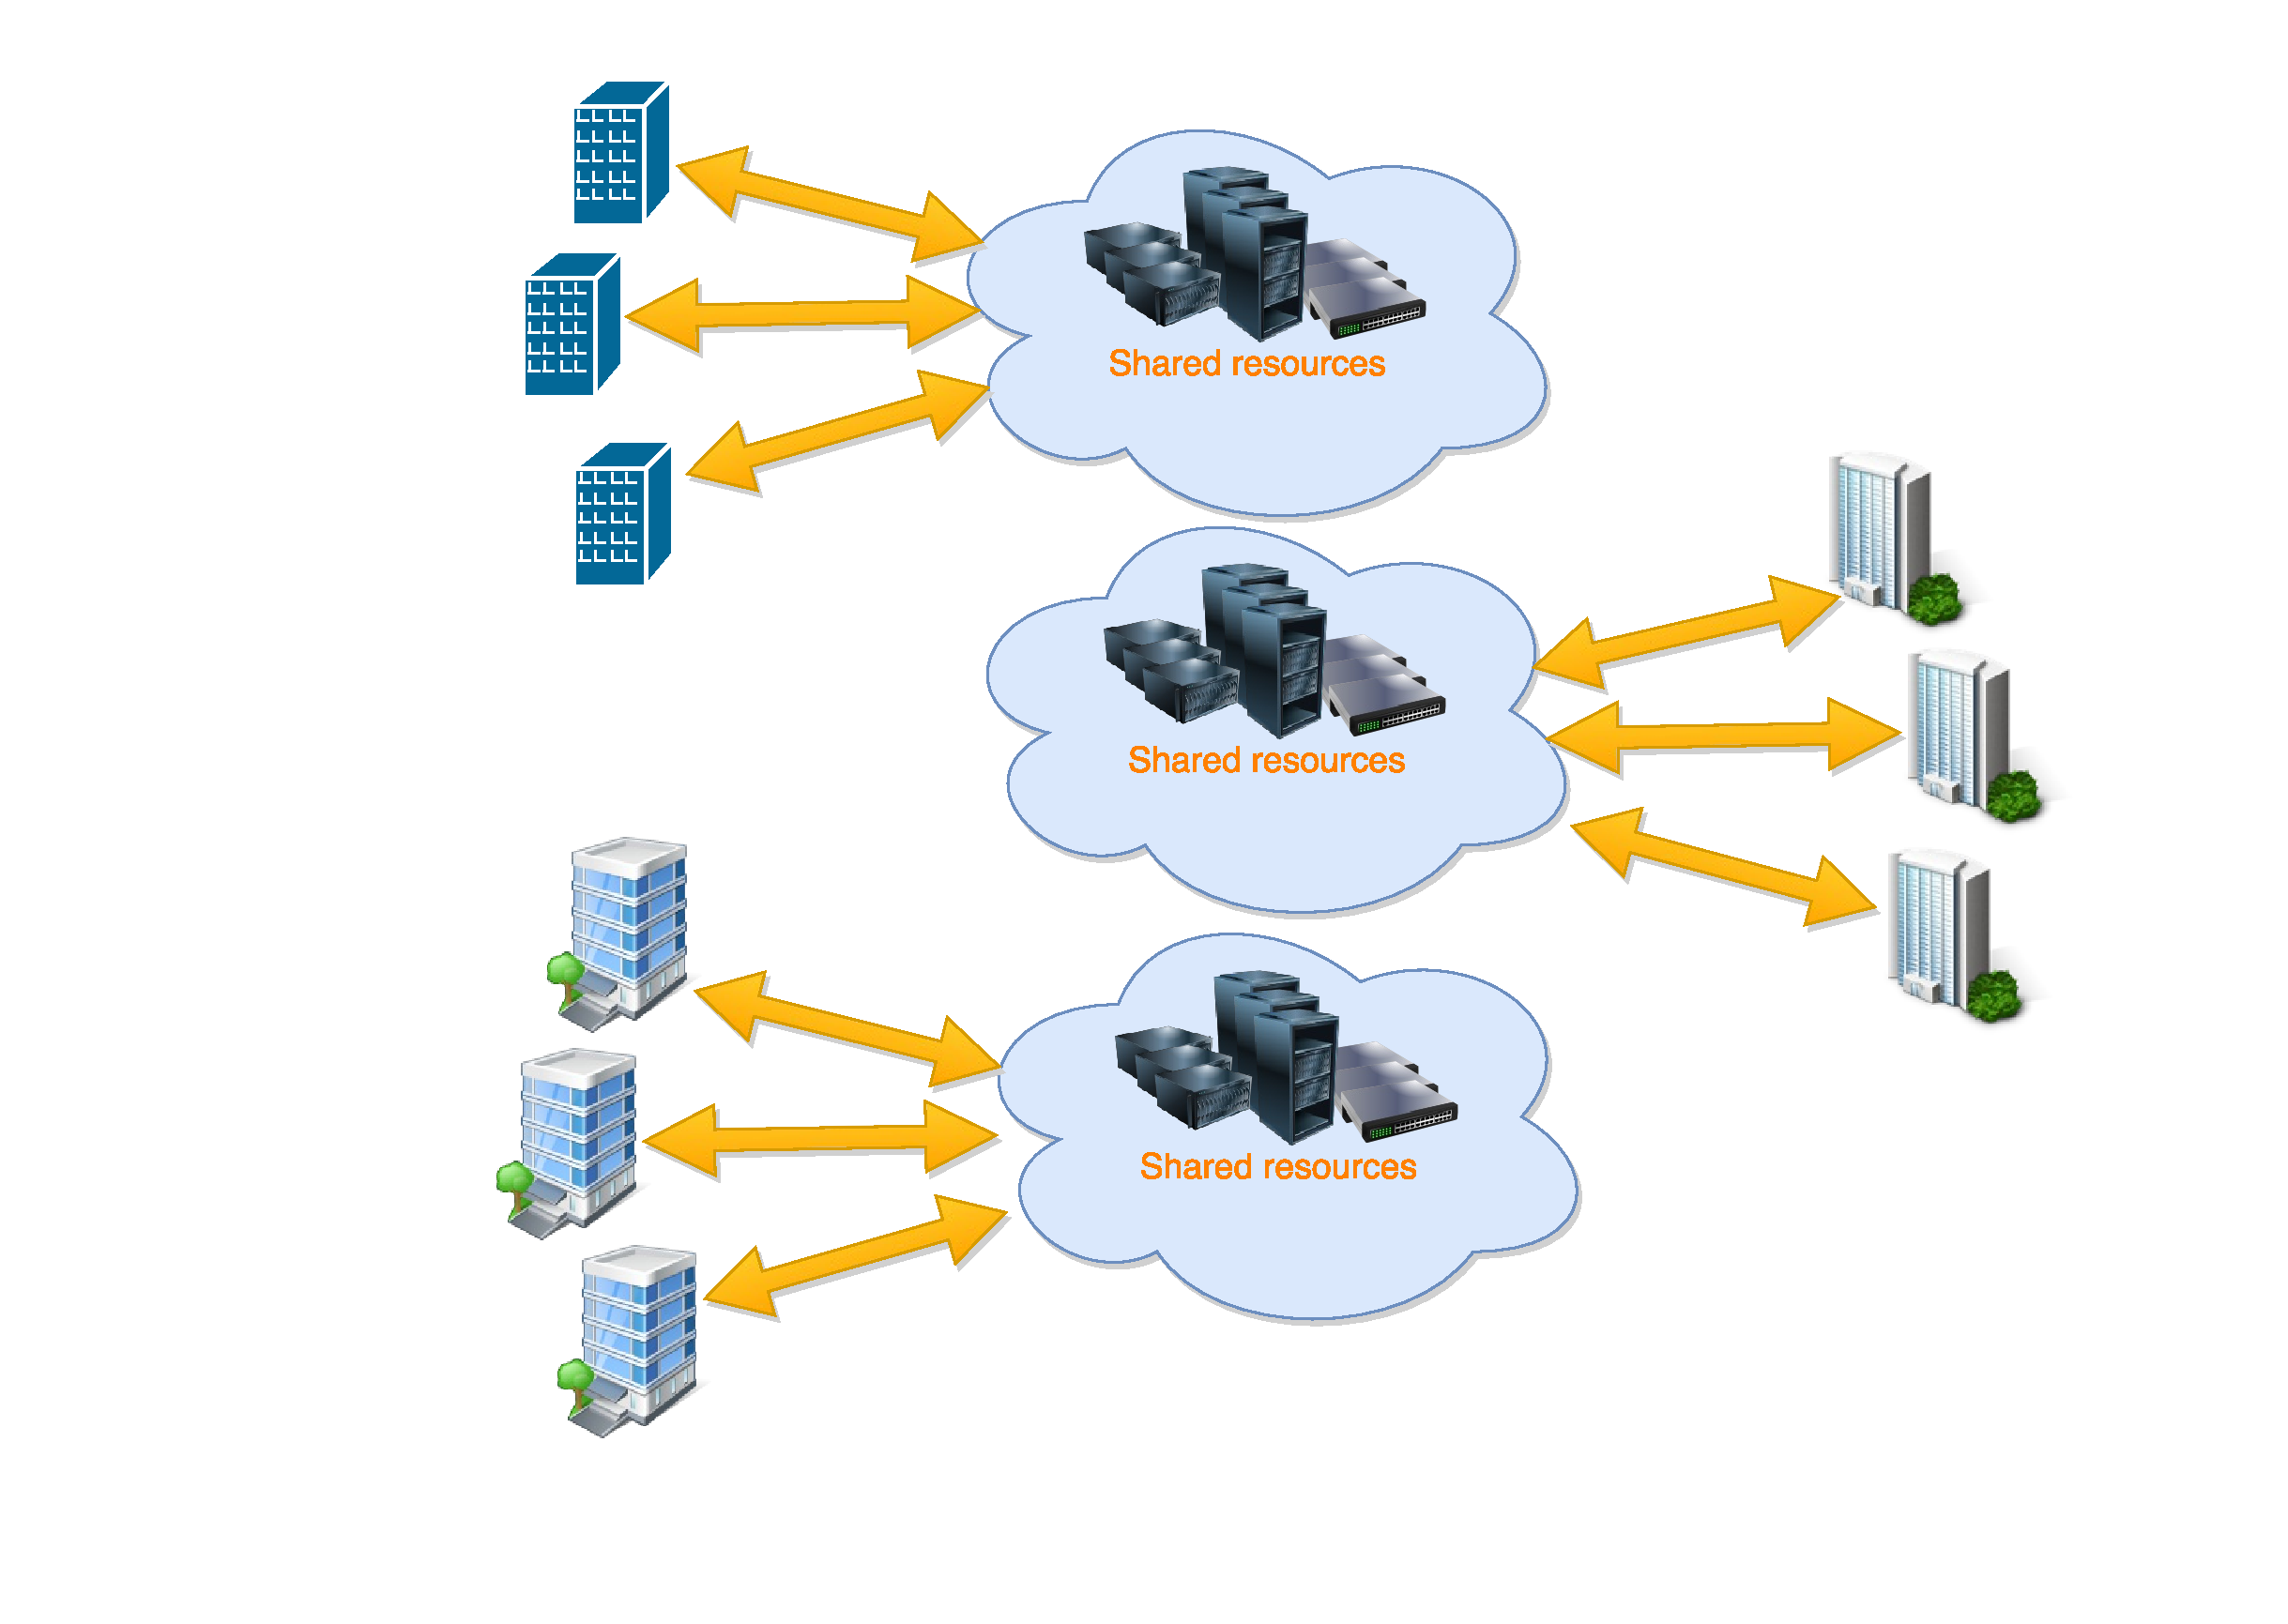
\includegraphics[scale=0.3]{communitycloud.pdf}
\caption{A high level community cloud architecture}
\end{center}
\end{figure*}
\subsection{Service models}

\paragraph{Software as a Service (SaaS).}
Consumer can use provider's  application which is running on a cloud infrastructure. As mentioned earlier, consumers can access provider's application through various devices and from various locations. Basically, consumer need a device with a web browser or provider's user application installed on it, and an internet connection. Consumers using SaaS, do not manage or control the underlying infrastructure of the application such as networking and storage. Service provider should handle all the responsibilities of this kind. So, consumers do not have control over the core settings of the application. 

\paragraph{Platform as a Service(PaaS).}
PaaS model is a very useful model mainly for developers. In this model, consumers develop and deploy their applications by using development tools which are provided by the service provider. This model is very suitable for enterprises which are not wishing to invest in development tools. Tools like programming languages, libraries, service and related licences are provided and supported by the service provider. As in the case of SaaS, Consumers do not have control over cloud's underlying infrastructure such as networking and storage. In PaaS, consumers have control over setting of their own developed applications deployed in the cloud. 

\paragraph{Infrastructure as a Service (IaaS).}
This service model enables consumers to provision infrastructure related resources such as storage, network and computing resources. Basically, consumers have the capability to run any desirable software on the assigned systems. The full control of operating system of the assigned machines are with the consumer. As previous models, consumer do not have control over the underlying cloud infrastructure. 

\subsection{Threats associated with cloud computing}
Cloud computing has transformed service computing and businesses. The way that cloud computing delivers computing, has opened various new business opportunities. Shifting to cloud computing is fast but at the same time it should be with caution. As there are various benefits in the cloud for consumers, more and more consumers are moving their data, processes and computations to the cloud. At the same time malicious parties are specifically focusing to the cloud too. So this movement of attacks and attentions toward the cloud, reveal several threats that threaten security and privacy of users data. \\

Some of threats toward the cloud either arise because of cloud's essential characteristics (mentioned in previous sections) or cloud's core technologies. Basically cloud computing is comprised of several core technologies. Three cloud main technologies are: cryptography, virtualization and web applications and services  \cite{ref9}. To a large extend, cloud computing depends mainly on the mentioned technologies.  Specifically, some of service models which will be discussed later in this Chapter, are deliverable through web applications and services. On the other hand ,the whole cloud is built on virtualization technology, particularly its infrastructure service. Third technology which is cryptography, is the solution to many cloud computing security and privacy problems. \\

A threat can be related to the cloud if, it's root cause is in one of the cloud's characteristics mentioned earlier or the threat is prevalent in one of the cloud's core technologies \cite{ref9}. In other word, a vulnerability that threaten security of the virtualization, definitely threaten security of the cloud too.\\

Based on \cite{ref1}, nine top threats to the cloud which should be seriously addressed specifically by researchers are in the following:
\begin{itemize}
\item Data breaches: It is very important that sensitive data of any information remain secret and not to be known by non authorized parties. Multi-tenancy (specifically in public cloud deployment model) opens a venue for this threat to take place. Vulnerabilities in shared applications can put data of all consumers of that specific shared application in danger. One of the prevalent solutions to mitigate against this threat is using encryption technologies. On the other hand, encryption technologies are also prone to attacks.    
\item Data loss: This point refers to actions that need to be taken by both service user and provider to prevent loss of data. Examples of these actions are back up and disaster recovery policies. Data in the cloud can be lost due to reasons other than malicious activities. An example of those reasons can be natural disasters. Generally, consumers should be responsible for having backup of their own data while service providers should be responsible for taking preventive actions to reduce probable losses.  
\item Account or service hijacking: This point is not cloud specific as it happens in conventional environments too. The difference is by gaining access to specific cloud accounts, attacker may have access to vast amount of private data and infrastructure.
\item Insecure APIs: Cloud's consumers use from several cloud services through APIs. These APIs are provided to them by service providers. Consumers use APIs to manage their resources. APIs should be protected no to be misused by malicious users to access to critical data of users. 
\item Denial of service: As users of cloud resources primarily have access to services through standard internet connection, availability of the services is vital. So, any obstacle that prevents network connections between consumers and online resources, prevents users to access their data through other means like local access in conventional environments. DDoS attack toward CSPs can prevent consumers to have access to their data. This matter can cause financial losses to both CSPs and consumers.   
\item Malicious insiders: System administrators and CSP's employees that have access to cloud's resources may misuse their privileged access. Adequate access control methods should be applied by CSPs to prevent probable misuses.
\item Abuse of cloud service: Cloud computing offers a great amount of on demand and scalable resources to all kind of consumers. In some cases, malicious consumers can misuse the vast amount of resources for variety of malicious activities. It is vital for CSPs to detect misuses from their resources and prevent them from happening. 
\item insufficient due diligence: This point is a less technical threat compared to other threats. It refers to lack of consumer's knowledge about the cloud environment in which they are willing to move to. The environment refers to CSP, application or a cloud service. 
\item Shared technology issues: CSPs deliver their services through sharing underlying resources. As mentioned earlier, vulnerabilities in shared resources can threaten security of all consumers using the same shared resource. 
\end{itemize}

\subsection{Risk associated with cloud computing}

While some consumers move their data to the cloud, other consumers are in doubt. The doubt arises from risks associated with cloud services. That is the reason that cloud risk assessment studies are developing. Based on \cite{ref39}, cloud computing offers various opportunities (specifically for small to Medium Enterprises) and advantages. Opportunities that are discussed here are mostly network and information security opportunities. Some of these opportunities are: Backups; Certification and compliance; standard formats and interfaces and physical security. There are some risks associated with these opportunities. Some of these risks are consequences of the cloud related threats. In \cite{ref39}, eleven risks are mentioned for the cloud. The risks associated with cloud are in the following:\\
\begin{itemize}
\item Software security vulnerabilities 
\item Network attacks 
\item Social engineering attacks 
\item Management GUI and API compromise  
\item Device theft/loss 
\item Physical hazards 
\item Overloads 
\item Unexpected costs 
\item Vendor lock-in 
\item Administrator or legal outage 
\item Foreign jurisdiction issues 
\end{itemize}

\section{Virtualization}
Virtualization is a software technology which enables multiple operating systems and applications to run on a same server (host) at the same time. Virtualization is an effective way to reduce IT related expenses and to increase efficiency. It is effective for both large and small enterprises. Virtualization is some sense is the heart of cloud computing. Virtualization refers to virtual forms of various physical devices. Virtualization applies to computer hardware, storage devices, operating system, applications and networks too. Virtual computer systems are called the Virtual Machine (VM). Each VM consist an operating system with various applications. VMs are independent from each other. Using virtualizaiton has various benefits. Some examples of benefits of virtualization consumption are in the following: \\ 
\begin{itemize}
\item Reduction of operational costs dramatically 
\item Increase productivity and efficiency
\item High availability for applications and services through provisioning
\item Enable a central management through simple systems
\end{itemize} 

A layer which is placed between VMs and the host called hypervisor is responsible for operation of VMs and allocation of physical resources to them. VMM or hypervisor is a software that runs VMs and manages resource allocation to them. The system on which VMM runs is called host. VMMs are either bare-metal or hosted. In case of bare-metal, VMM runs directly on the underlying hardware. In case of hosted, VMM operates on an operating system. There are a variety of commercial and open-source versions of VMMs. \\

One of the open-source VMMs that we also used for our implementation  is Xen. Xen \cite{ref18} is an open source and widely used VMM. VMs running on Xen are referred as domains. There are two domain types in Xen, privileged domain and unprivileged domain. A supervisor like VM, called Dom0 runs as privileged domain. VMs running on Xen should run either on Hardware Virtualization (HVM) or Para Virtualization (PV) mode. In HVM, VMs are not aware that they are running in a virtualized environment, whereas in PV mode, VMs experience some modification and are aware that they are running on a virtual platform.
 
\section{Botnet and BotCloud}
Botnet refers to a group of computer systems that are infected with a piece of malicious software. The malware allows the controller (bot master) to take control of various parts of infected systems and take specific arbitrary action. Victims are not aware of the actions which their system take in favour of the bot master. Infected machines are called zombie. The program that is responsible for infecting victim's system is called bot. As bots tend to remain hidden, rootkits are used for their activities. There are various methods that bots can infect victim machines. Spreading pirated software is one of the prevalent ways. Malware authors try to hide their malicious software inside pirated software. At the time which victims install the pirated software, bots leave their effects on the systems too. Another way to spread the malicious bot software is through Email and spamming. \\ 

At the time of installation, Bot software installs a backdoor on the system of the victim. The backdoor enables botmaster to communicate with victim's machine. Through the backdoor, botmaster is able to send commands to the zombies and even send updates and newer versions of the malicious code. As mentioned earlier, some of activities that botnets are able to do are: DDoS attack, spamming, search engine optimization poisoning, pay-per-click fraud, financial fraud, bitcoin mining and information stealing \cite{ref22}. \\

Botclouds are botnets that are formed based on a CSP's resources. Botcloud misuses cloud's legitimate resources to conduct malicious activities. Some of the cloud's characteristics allow attackers to form botclouds much easier than forming botnets in conventional environments. On the other hand, CSPs allow consumers to have access to a vast amount of resources with very low prices. So botmasters tend to form botclouds compared to forming botnets.  

\begin{figure*}
\begin{center}
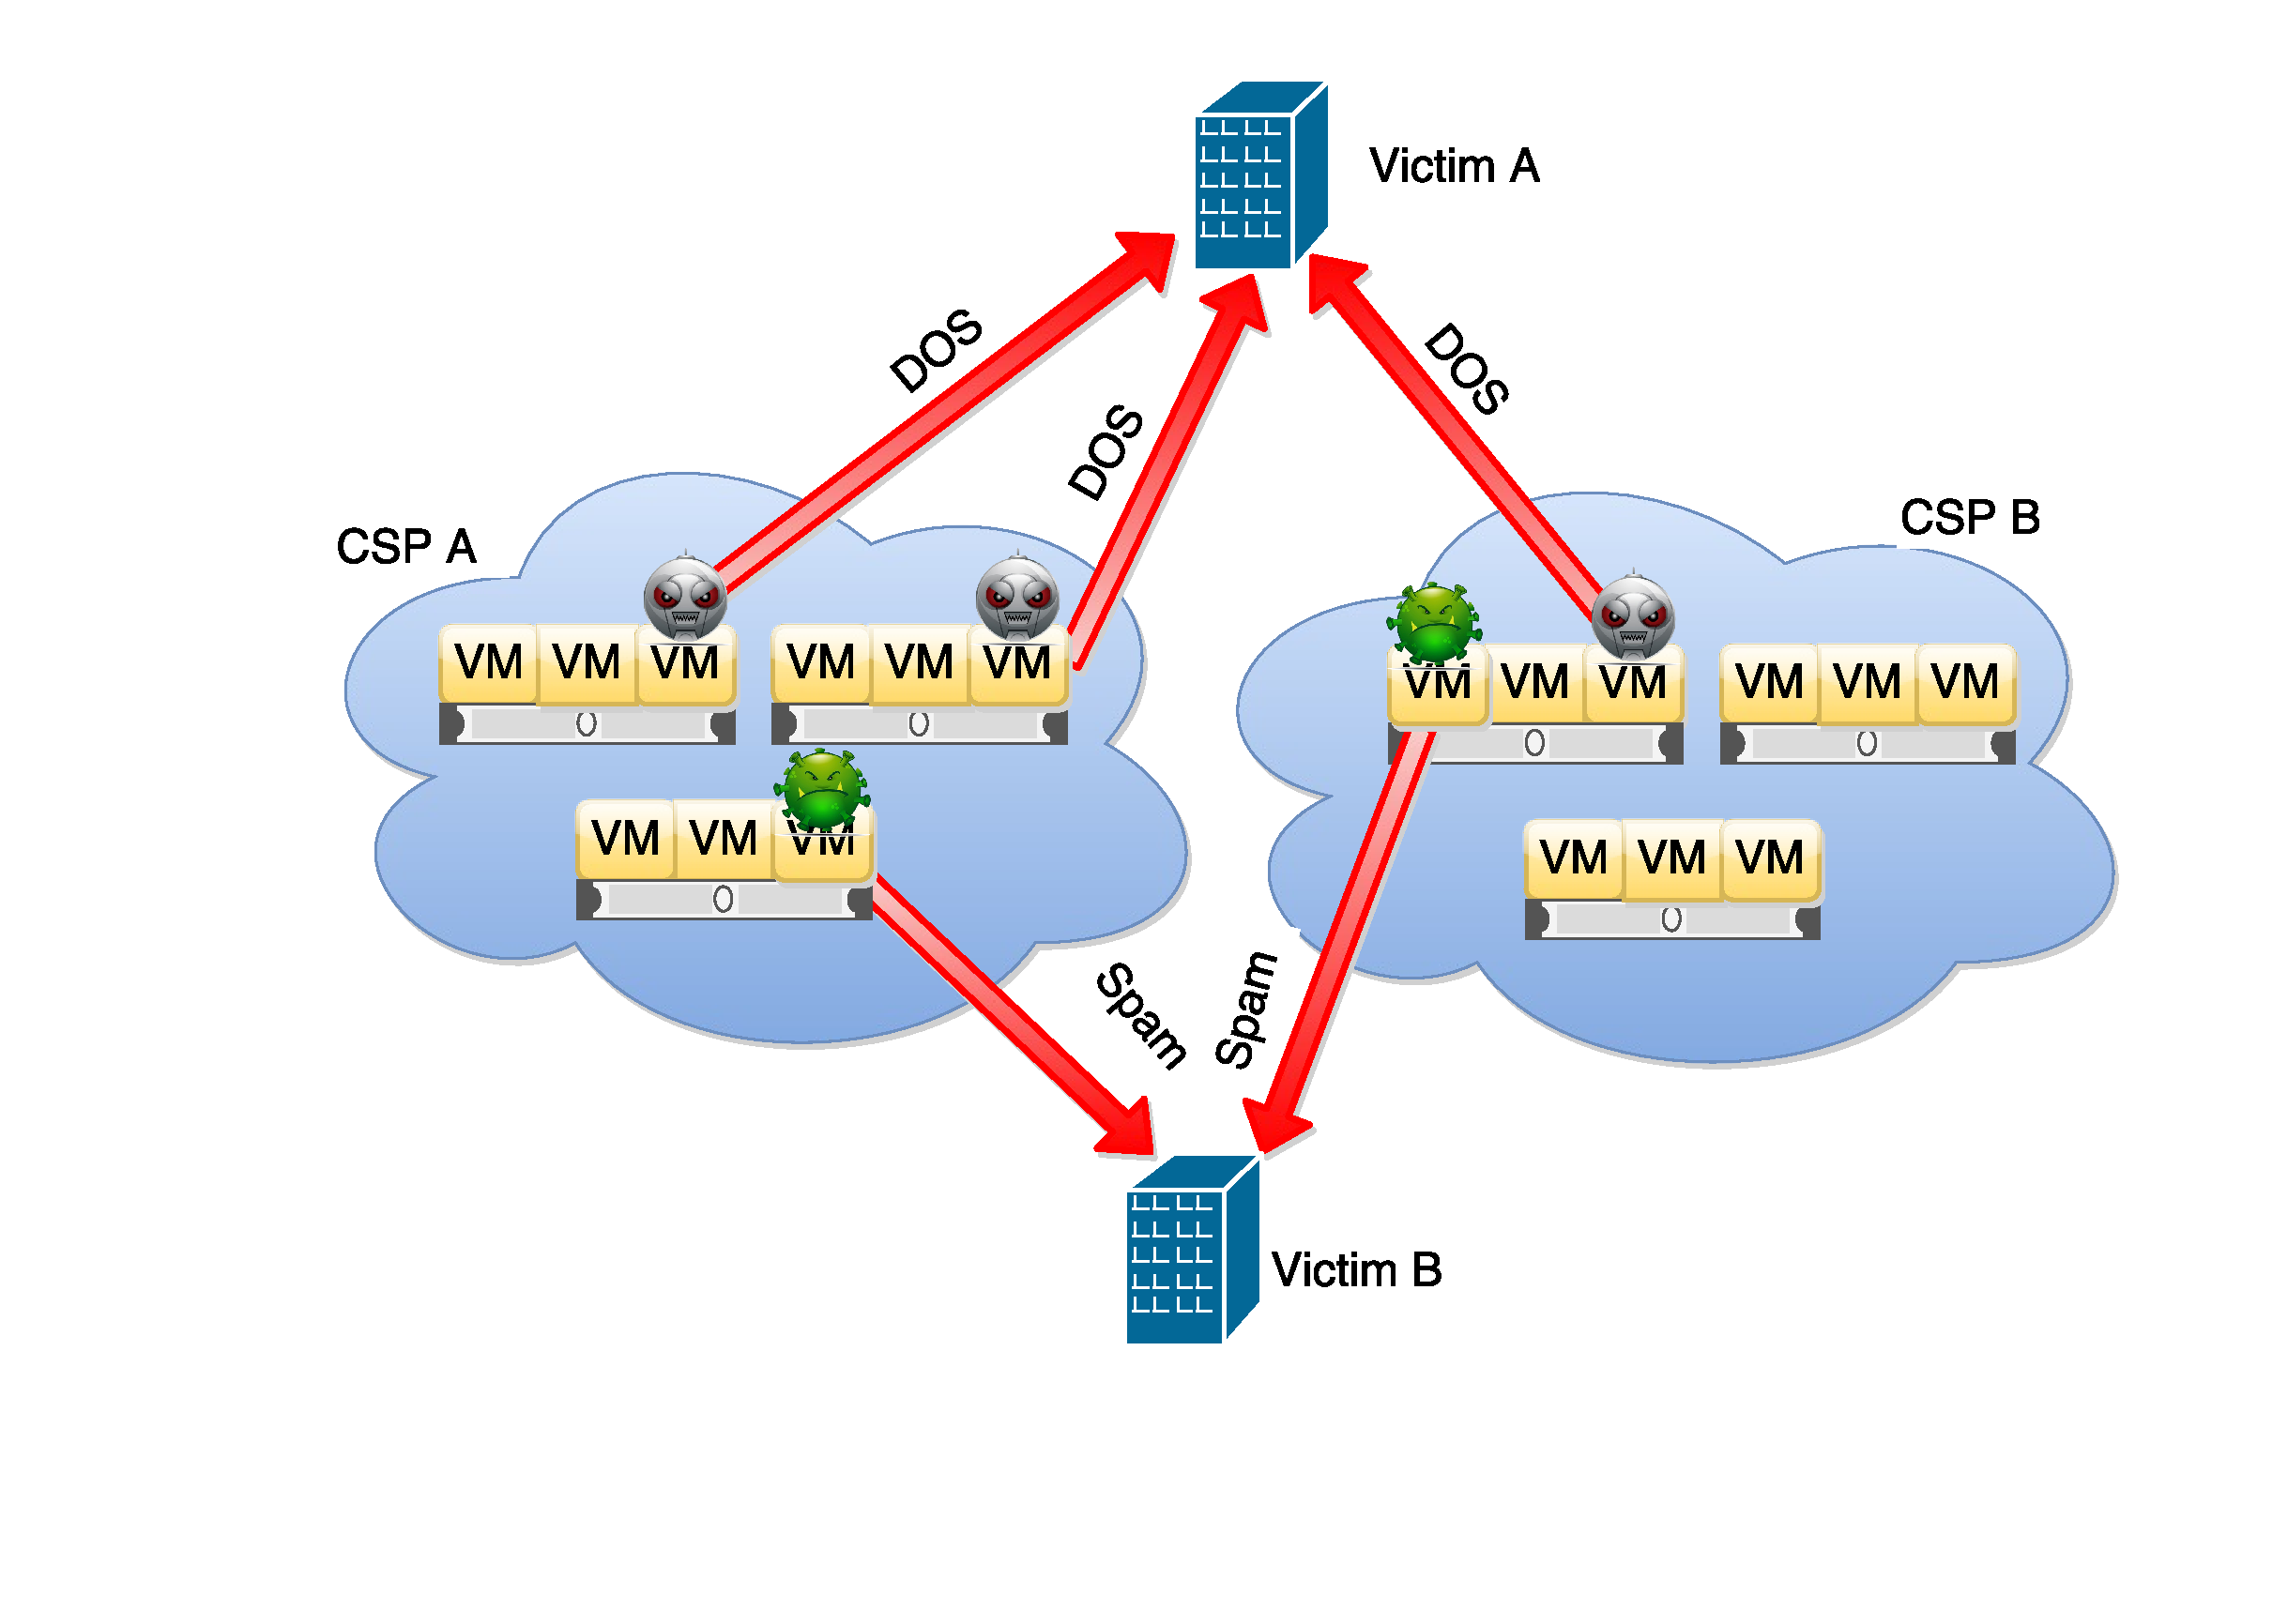
\includegraphics[scale=0.3]{botcloud.pdf}
\caption{A botcloud figure}
\end{center}
\end{figure*}

\section{Virtual Machine Introspection (VMI)}
VMI is a technique used in virtualization to inspect memory space of a VM in real time. Inspection takes place from a secure point which can be another VM (i.e., Dom0) outside of the inspected VM. In this way, there is no need for installation of local agents on each introspected machine. Agentless manner has the benefit of increment in security. In agent oriented systems, malicious code might disable the security software or the related agent in order to escape detection. Since VMI takes place through an agent less procedure, this threat is mitigated. VMI technique is applicable to security monitoring systems which operate within virtual environments. \\

To conduct introspection, an appropriate Application Programming Interface (API) to use is LibVMI \cite{ref11}. LibVMI which currently is usable with XEN and KVM, enables introspecting VM to read from and write to memory of introspected VM. Introspection through VMI is done in an agent-less manner. LibVMI is well integrated with Volatility \cite{ref19}. Volatility is an advanced open source memory forensic framework which offers variety of functions to users for extraction of data from memory snapshots and dumps. As LibVMI has integrity with Volatility, it is possible to use Volatility functions on live VMs while using LibVMI. It happens by adding the LibVMI address space to the address space list of Volatility.

\begin{figure*}
\begin{center}
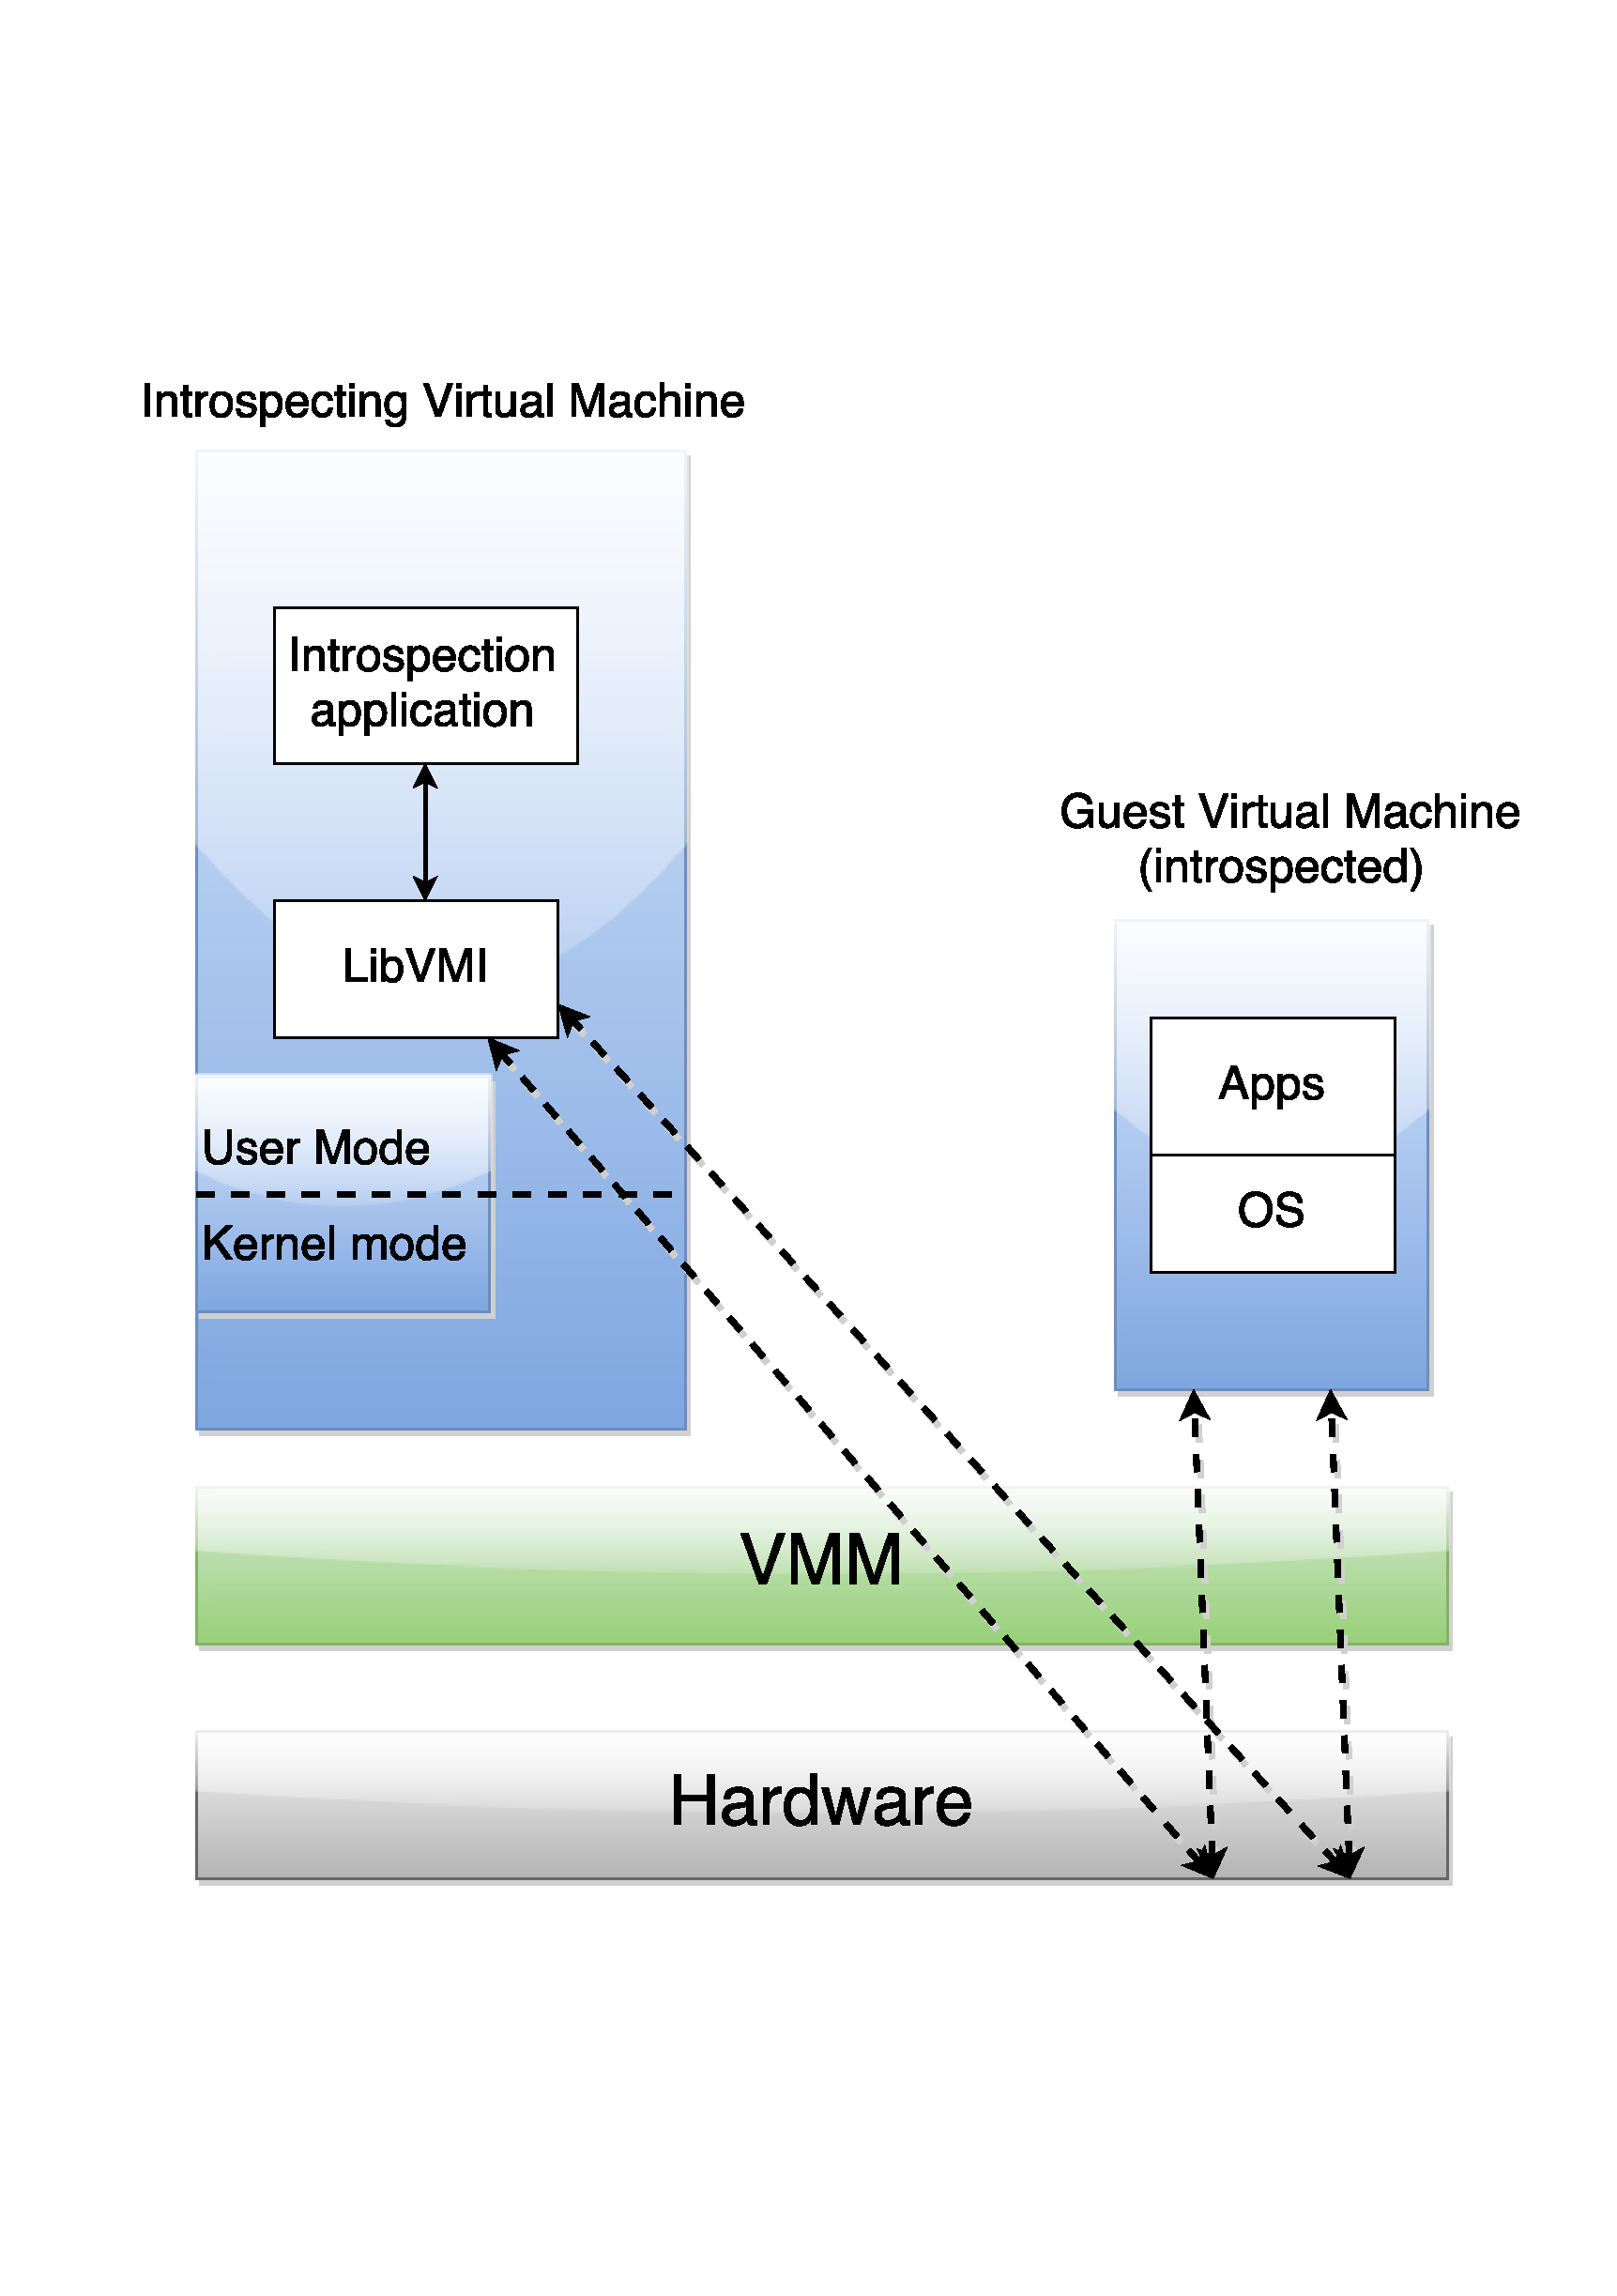
\includegraphics[scale=0.3]{vmi.pdf}
\caption{Using introspection to obtain internal Vm's data }
\end{center}
\end{figure*}


\chapter{RELATED WORK}
In this Chapter, we discuss previous works done on botcloud detection and malware detection in the cloud using VMI.
 
\section{Botcloud detection}
As mentioned in Chapter 2, botclouds are different from conventional botnets in various ways. So detection of them requires some considerations. That is why we mostly focus on previous works done on detection of botclouds instead of botnets in conventional environments.\\

Kebande and Venter \cite{ref3} presented an approach to detec botnet in the cloud environment using Artificial Immune System (AIS). This mechanism uses a negative selection algorithm. Through this proposed process, authors clain to be able to detect the probability of botnet infection based on the process of independent Poisson process and detection
based on negative selection. Researchers in \cite{ref41} proposed the botcloud source detection approach which aims to detect abnormal VMs behaviour. The proposed detection approach is based on principal component analysis and focuses on behaviours that support DDoS flooding attacks. \\ 

Researchers in \cite{ref4} designed a passive and an active detection module in VMM to look for information in VMs using VMI and profiling bots. Their work mainly focuses on functions in one host and detects infected machines, based on trained node about bot behaviours. They make the botnet profile based on just the API calls done by the applications. Francois et al., in \cite{ref2} address botnets that rely on peer to peer networks for communication. They propose a distributed framework that leverages a host dependency model and an adapted PageRank algorithm. \\ 

In \cite{ref5}, researchers present an approach that enables a source-based detection of UDP-flood DDoS attacks. Their system's detection logic is based on a distributed system behaviour analysis. As \cite{ref41}, In this work the detection is based on a principal component analysis. \\

\section{Malware detection in the cloud specifically using VMI} 

Garfinkel and Rosenblum in \cite{ref10} proposed use of VMI as an enabler for intrusion detection tools. They correctly addressed the problem that IDSs must reside on VMs to have an excellent view of interior of systems. In that way, IDS can be target of attack by the malicious software that infects the system. Furthermore they presented their detection system equipped with VMI. Researchers in \cite{ref8}, propose a multipartition, multichunk ensemble classifier. The multipartition, multichunk ensemble technique helps to reduce classification error.\\

 Watson in \cite{ref13} presented a distributed detection system design that detects spread of malware in multi-server cloud. This work presents a method of detection based on a distributed network of detection agents. This work takes place in order to coordinate detection across the whole cloud. This would provide a mechanism for locking down vulnerable VMs in the event that malware is detected in the cloud. Beidermann and Katzenbeisser in \cite{ref12} presented a research work to detect computer worms in the cloud based on the spreading behaviour. Their solution looks for inconsistencies in behaviour of machines. The claim that their system is able to detect unknown and new appearing computer worms. As mentioned, their proposed system detects spread ing worms based on spreading behaviour. \\

Harrison et al., in \cite{ref6} presented a framework for malware detection in the cloud by using symptoms. They present a method of detecting malware by
identifying the symptoms of malicious behaviour as opposed to looking for the malware itself. Researchers in \cite{ref7}, presented tiny VMs called Forensic Virtual Machines (FVMs) to gather information via VMI for detection of malicious activities. Each FVM searches for existence of a specific symptom of malicious activity in a VM. After inspection, the FVM chooses a random VM and starts inspecting the newly chosen VM.



\chapter{EYECLOUD DESIGN}
In this section, we present our approach toward EyeCloud design. In particular we focus on monitoring (Section IV.A), detection (Section IV.B) and reaction (Section IV.C) methods in addition to infrastructure architecture (Section IV.D).
\section{Monitoring method}
Data collectors gather relevant information in wide-spread manner. In our design, we use the concept of FVM for describing data gathering elements \cite{ref7}. As depicted in Figure 1, we assign one FVM per VM to extract system level information from each VM's memory pages at any given time using VMI. Each FVM is dedicated to one VM and looks for existence of all the required symptoms in the VM assigned to it. Assigning one FVM per VM as opposed to one FVM per symptom \cite{ref7}, has various benefits. Introspected VM should only trust to one FVM, which results in monitored VM's Trusted Computing Base (TCB) reduction. In addition, the symptoms are checked (frequently) all at once; this differs from state of the art approach considering only random checks. FVMs as any VM are not attack resilient. They might get infected too. In case of a FVM infection, other monitored machines can remain immune. On the other hand, for deploying the system in large scale, overhead and scalability issues arise. The discussion about these issues are beyond the scope of this paper, and we will consider them as future work.    
\begin{figure*}
\begin{center}
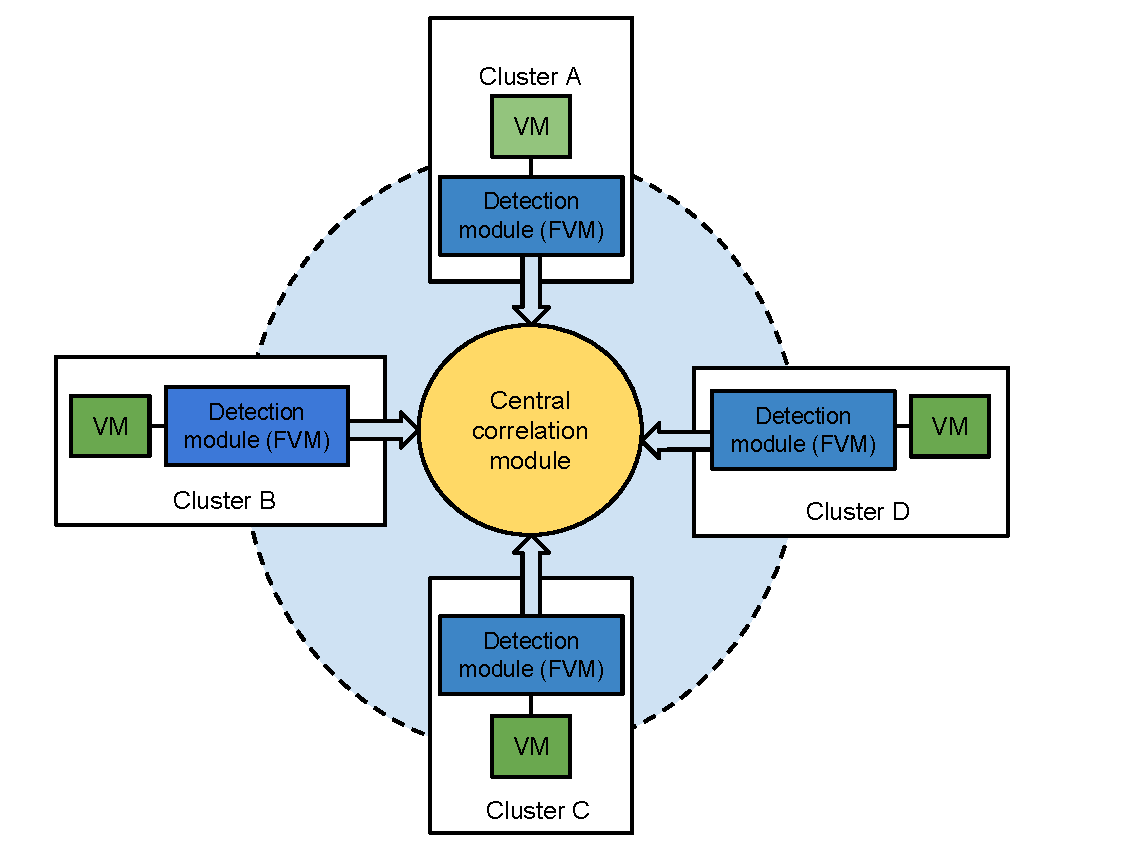
\includegraphics[scale=0.6]{pic111.pdf}
\caption{A wide-spread data collection with central correlation}
\label{Fig:111}
\end{center}
\end{figure*}
Figure 1 depicts a high level design of EyeCloud with FVMs incorporated in it. FVMs collect data and transfer them to central correlation module. By comparing the EyeCloud design and a typical cloud platform design, cloud controllers can be hosting units for central correlation modules. The reason is because the cloud controller is the outermost entity in a cloud platform design. So, in order to discover distributed attacks on VMs, FVMs do not have to participate in event correlation. This helps to make FVMs lighter. Apart from the method that is used for data collection, determination of what is actually collected is vital. A sample list of symptoms can be defined by determining inconsistencies in an infected VM. We consider Windows operating systems and we focus on system level inconsistencies (i.e., inconsistencies mentioned in Table I). \\

Based on \cite{ref20}, we prepared Table I which depicts common modifications that nine botnet related malwares cause to victim's system. Under each malware's name, the year that malware was discovered is mentioned. By looking at Table I, we conclude all the listed malwares create registry entries. As a result, creating registry entry is a prevalent action among listed malwares. Hence, creation of registry value under a specific key would be a symptom as opposed to the registry entry value. To reduce false positive, one should look for a set of diverse symptoms. So occurrence of number of diverse symptoms among several machines would trigger security alert while revealing differences among VMs.\\

Based on \cite{ref43}, \cite{ref44}, \cite{ref21}, \cite{ref35} and Table I, a set of inconsistencies that we consider is the following; \\

1) \textbf{Existence of hidden processes}. Existence of an abnormal process in the process list is rare by advanced malware as their existence will be revealed easily and fast. On the other hand there is an alternative option for malware authors to inject the malicious code into legitimate processes. Hence, relying solely on the name of running processes in the process list is not a  potent method toward detection of malicious software. Another alternative for rootkits, is to unlink the malicious process from the process list's linked list causing the malicious process not to be present in the list of running processes. A process usually is not unlinked from the linked list of processes, unless there would be possibly malicious activities at the back of it. 

2) \textbf{ Shutting down security mechanisms - Firewall}. In case of Windows operating systems, one of the security mechanisms that can be target of attacks is Windows firewall. Windows firewall can be disabled for legitimate purposes too, but appearance of this symptom beside other symptoms can be a potentially malicious act.

3) \textbf{Inappropriate commands in history of the command shell}. Adversary may have direct access to the shell of a system and run some commands directly through the shell. One of the use cases for this matter is when adversary has access to the shell and he can install a service through the command line. 

4) \textbf{Existence of hidden DLLs}. Existence of a hidden DLL (unlinked) is another technique that can be used by malicious codes. There is possibility that the DLL is injected into other processes. This possibly requires a new view toward malicious DLL detection. 

5) \textbf{Shutting down security mechanisms - Windows defender}. As we focus on Windows operating system, Windows defender is one of the vital services that should be checked against getting disabled specifically in Windows 7.

6) \textbf{Shutting down security mechanisms - Automatic update}. As updates and patches are necessary for systems to remain secure, automatic updates may be target for being shut down. 

The main audit source location is each VM's memory using VMI technique. Using VM's memory as audit source location aims to reveal hiding of low-level local activities while identifying actual attacking entities. 

Time of detection is in real-time manner. An infected machine is detected to be infected by the correlation element after an actual infection has occurred. The actual infection may not necessarily result as an immediate damage. As the EyeCloud detects malicious VMs based on system symptoms as opposed to behavioural analysis, it can prevent further damages to systems and networks.  
\section{Detection method}
EyeCloud's detection logic is based on clustering. Clustering is one of the data mining techniques. Data mining is a wide-spread analytic technique. Clustering is one of the notable branches of data mining that is based on unsupervised learning techniques. Unsupervised learning is finding structures out of unlabelled data sets. \\

In EyeCloud's design, we aim to group a set of VMs into subsets such that all elements in each subset group are more similar in comparison to elements in the other group. One group would contain infected VMs while the other would contain clean elements as grouping occurs based on inconsistencies determined earlier. The novelty of the combination of all the solutions is that based on general symptoms and regardless of type of malwares, VMs are grouped. So by using a clustering technique, it would be possible to identify a set of VMs that are infected by different malwares. 


\begin{table*}[ht]
\centering
\small
\def
\arraystretch{0.8}
\begin{tabular}{|m{2.5cm}|C{1.3cm}|C{0.7cm}|C{1.1cm}|C{1.0cm}|C{1.1cm}|C{1.0cm}|C{0.7cm}|C{1.2cm}|} \hline
System modification & Rustock.B (2006)&Virut (2007)&Koobface (2008)&Tidserv (2008) &Qakbot (2009) &Pilleuz (2009) &Zbot (2010) &Carberp.B (2014) \\ [0.9ex]\hline
File created (under certain directories)  & \checkmark &  &\checkmark &\checkmark &\checkmark &\checkmark &\checkmark &\checkmark \\ [0.9ex]\hline
File Deleted  &  &  & &\checkmark &  &\checkmark &  & \\[0.9ex] \hline
File Modified & & \checkmark & &\checkmark &\checkmark &\checkmark & & \\ [0.9ex]\hline
Registry entry created (under certain keys) & \checkmark &\checkmark &\checkmark &\checkmark &\checkmark &\checkmark &\checkmark &\checkmark \\ [0.9ex]\hline
Kernel modification & \checkmark &&&&&&&\\ [0.9ex]\hline
Code injection into process/DLL/App & \checkmark &\checkmark &\checkmark &\checkmark &\checkmark &\checkmark &&\\ [0.9ex]\hline\end{tabular}
\begin{center}
\caption{Botnet intended malware functionalities based on \cite{ref20}}
\end{center}
\end{table*}


Using general symptoms as attributes for clustering algorithm has benefit of reducing signature based technique rules of misuse detection while increasing detection rate. The mentioned technique would increase likelihood of new malware to be detected because system would not need to be updated frequently as signature based systems. On the other hand, there might be false positives too. In our method, likelihood of detection and rate of false positive, heavily depend on the symptoms which are chosen to be checked by detection modules.      

\section{Reaction method}
There are two reaction methods that are applicable to the EyeCloud. They are passive and active reaction methods. A passive response does not take correction action against attacking entities. It takes actions such as notifying an administrator. While active response takes corrective actions such as modification of attacking entity. \\

EyeCloud has both passive and active response types. Looking at Figure 2, passive method is achieved when analysis and clustering module notifies the alarm and report module about its decision. Administrators are required to analyse the obtained figures and results in this level. Active mode is achieved by the central correlation unit communicating with the VMM of the physical machine holding the infected VM. Central correlation unit can issue a command to the VMM to freeze infected VM's CPU cycle.
\section{Infrastructure}
A collaborative detection system consists of several detection elements where each consists of two main components, detection and correlation modules. By getting idea from Software Defined Networking (SDN), we only hold detection modules at the host level in the form of FVMs while having a single main correlation unit. So the EyeCloud can be categorized as a collaborative detection system. \\

As depicted in Figure 2, the data collected by each FVM gets in a relevant data structure by symptom search modules. This module only indicates existence or non-existence of symptoms in VMs. The data goes to the central correlation module located in the cloud controller through the VMM. Indeed by placing a detective module in the cloud controller level, analytic task gets offloaded from the VMM. As FVMs only collect and pass the data, a separate database is not necessary at their level. A global database is considered in order to communicate with the central correlation unit. Administrators can retrieve different stages of clustering results from the central database.\\

As depicted in Figure 2, seven components are in EyeCloud design. Each component is described shortly in the following:

\begin{itemize}
\item Authentication: List of legitimate users are stored in the central database. Administrators that must have access to the core, are authenticated through authentication module.    

\item Data collection: Information from VM's memory is collected through data collection component. Data collection takes place based on the symptom list that is available in core. Data collection module should retrieve the list from core.  

\item Symptom search: Collected information should be analysed to check to determine status of a symptom.  

\item Analysis and clustering: This component analysis the data set using K-Means algorithm of data mining. Based on information available in dataset about VMs, each VM is  assigned to one group (cluster). 

\item Core: Legitimate users should connect to the core in order to view the result of analysis done. So this component is working as user interface too. Users can issue command such as stopping a VM or freezing a VM's CPU through this component.  

\item Alarm and report: This component makes proper reports based on data received from Alarm and report component. It will send the reports and if probably issued to core. Core will show them to user.

\item Status save: This component help to save the current status that is shown by any time to users by the core component. There is a specific number of time that status are saved.  

\end{itemize}

To better understand various part of EyeCloud's functionality, we provide pseudocode of 3 main components. 
 
\chapter{IMPLEMENTATION AND EXPERIMENT}
In this section, we describe our implementation and experiment. In particular, in the first subsection (Section V.A) we describe implementation details. In the second subsection (Section V.B) we explain our experiment details.
\section{Implementation}
As for testing the idea that this research is built on it, we set up a test environment. We mainly focus on depicting the possibility of required data collection with desired tools and libraries in order to provide the collected data to clustering algorithm. Furthermore to show that based on the chosen attributes, it is feasible to separate infected VMs from others. \\

As the hardware, we used a Dell laptop model Latitude E5440 that consists 8 GB of RAM and an intel core i5 processor. On top of the hardware, we set up a virtualized environment. We used Xen version 4.4 as the VMM. Before setting up Xen, we needed to install an operating system which operates as the Dom0 operating system. Based on experience, Ubuntu 14.04.2 LTS (Linux version 3.16.0-30-generic) was our choice for Dom0. So we set up a Xen 4.4 after we installed an ubuntu 14.04.2. Then we created several VMs running on HVM mode with the Windows 7 professional 32-bit as the operating system. \\

As for the introspection tool, we used the LibVMI version 4.4 to conduct introspection. To verify correctness of installation, several examples are provided by the library at time of set up which we ran them to verify correct installation. Next, we configured Volatility framework version 2.4 and connected it to our created live guest VMs. So we used Volatility in conjunction with LibVMI to collect required data by introspecting running VMs. For the sake of acquiring the needed data, we operated data collection from the Dom0 for this experiment.    \\

\begin{figure}
\begin{center}
\hspace{-1.5cm}
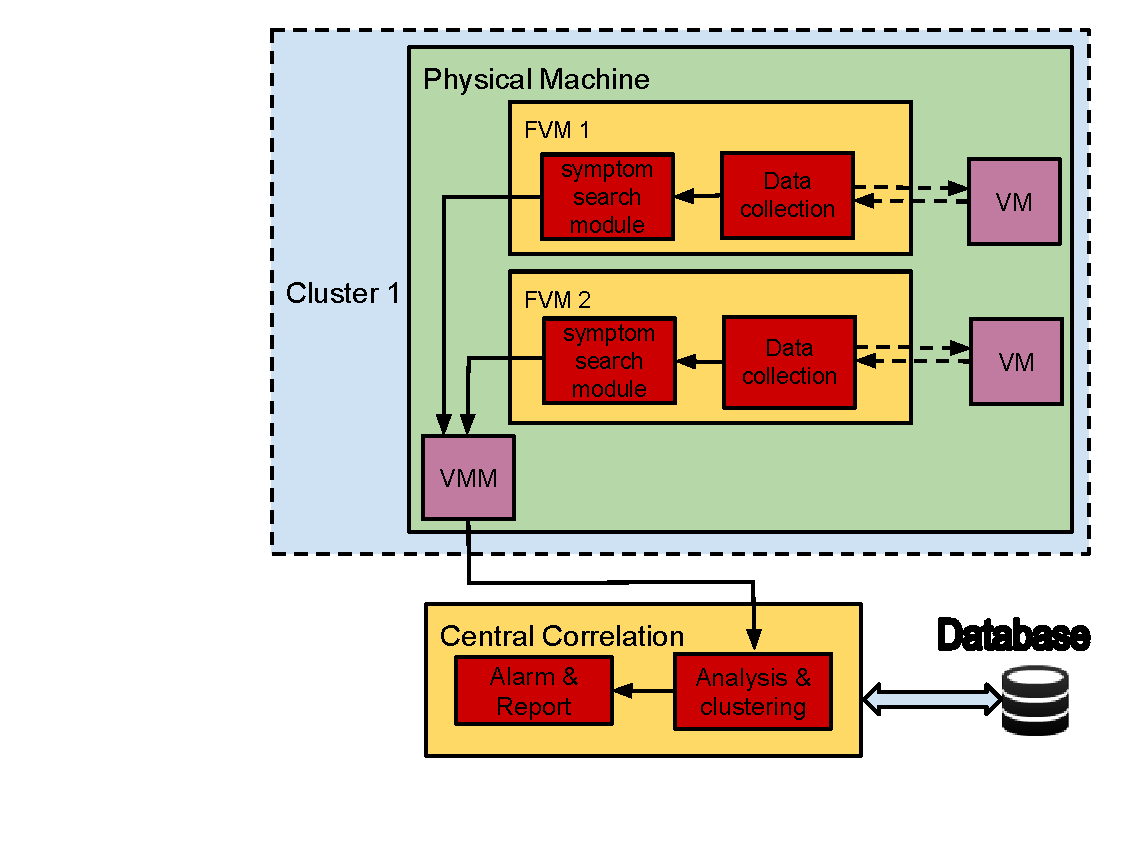
\includegraphics[scale=0.6]{pic114.pdf}
\caption{EyeCloud architecture}
\label{Fig:114}
\end{center}
\end{figure}

\section{Experiment}
For a simple illustration of feasibility of our proposed solution and based on our determined inconsistencies (attributes), we considered to collect data using VMI from 13 VMs. Looking at Table II, VM1, VM2, VM3, VM4 and VM5 are considered to be uninfected entities. The mentioned VMs are not infected by any kind of malicious piece of code. Meanwhile various conditions that may happen in non-malicious cases (i.e., shutting down firewall for a legitimate purpose) are considered. For instance we assumed VM2's user to disable one of the security controls of the VM intentionally for legitimate usage.   \\

As depicted in Table II, we infected VM6 through VM13 with various types of botnet related malware. We chose a sample of Zbot for VM6 and VM7, QAkbot for VM8 and VM9, Koobface for VM10 and VM11 and Pilleuz for VM12 and VM13. So there are pair of VMs infected by the same malware. The first pairs are assumed to have their security controls active, and the second pairs are assumed to have their security controls inactive. We acquired copies of malware that we used from online resources. Accuracy of the obtained malicious files were verified through a legitimate website \cite{ref45}.\\

For data mining section in the correlation module, we tested the collected data set over the K-means algorithm. For measuring distance between each data point and centroid in the k-means, we used the Euclidean distance algorithm as distance measure. If we assume K (user defined) to be the number of clusters and N to be the number of data points, then in our case, K=2 which is number of groups as well as number of centroids and N=13 (which is number of data points). \\

\begin{table*}[ht]
\centering
\def
\arraystretch{1.2}
\begin{tabular}{|m{1.2cm}|C{0.8cm}|C{0.8cm}|C{0.8cm}|C{0.8cm}|C{0.8cm}|C{0.8cm}|C{1.5cm}|C{1.0cm}|} \hline
&A.1 &		A.2 & A.3 & A.4 & A.5 & A.6 & Cluster index & Error\\ [1ex]\hline
VM 1 & 		0 & 0 & 0 & 0 & 0 & 0 & 1 & 0.125 \\ [0.9ex]\hline
VM 2 & 		0 & 1 & 0 & 0 & 0 & 0 & 1 & 0.875\\ [0.9ex]\hline
VM 3 & 		0 & 0 & 0 & 0 & 1 & 0 & 1 & 0.875\\ [0.9ex]\hline
VM 4 & 		0 & 0 & 0 & 0 & 0 & 1 & 1 & 0.875\\ [0.9ex]\hline
VM 5 &		0 & 1 & 0 & 0 & 1 & 1 & 2 & 0.72\\ [0.9ex]\hline
VM 6 &		0 & 1 & 0 & 1 & 1 & 1 & 2 & 0.52\\ [0.9ex]\hline
VM 7 &		0 & 0 & 0 & 0 & 0 & 0 & 1 & 0.125\\ [0.9ex]\hline
VM 8 &		1 & 1 & 0 & 1 & 1 & 1 & 2 & 0.32\\ [0.9ex]\hline
VM 9 &		0 & 0 & 0 & 0 & 0 & 0 & 1 & 0.125\\ [0.9ex]\hline
VM 10&		1 &	1 & 0 & 1 & 1 & 1 & 2 & 0.32\\ [0.9ex]\hline
VM 11&		1 & 0 & 0 & 0 & 0 & 0 & 1 & 0.625\\ [0.9ex]\hline
VM 12&		1 & 1 & 0 & 0 & 1 & 1 & 2 & 0.52\\ [0.9ex]\hline
VM 13&		1 & 0 & 0 & 1 & 0 & 0 & 1 & 1.375\\ [0.9ex]\hline

\end{tabular}
\caption{Collected data from VMs using VMI}
\end{table*}

\chapter{EVALUATION AND DISCUSSION}
In this section, we explain the obtained result of our cluster analysis. As depicted in Table II, each data point is assigned to a cluster. Data points which are grouped in cluster 1 are most of uninfected VMs and infected VMs that had security controls up. Data points that are grouped in cluster 2 are infected VMs that had security controls down. VM5 was not infected and is assigned to cluster 2 which is a false positive. Hence infected VMs that have their security controls off are separated as potential points of threat. This helps to reduce the target group under security analysis. As mentioned previously, result of clustering heavily depends on attributes. In our case attributes are symptoms. \\

Result of clustering analysis should be evaluated to measure its goodness. However good results of cluster evaluation do not necessarily depict a good result for a specific application. A simple evaluation criteria for cluster quality is purity. The maximum value of purity is 1 and the minimum value is 0. Purity result of 1 indicates a perfect clustering. The purity of cluster analysis for our system is 0.61 which is higher than average. Due to size limit in this paper, we skip the details of purity calculation. \\

Last column of Table II consists error rates for each data point. Error rate is the distance of a data point from an assigned cluster's centroid. Error rate's occurrences are depicted in Figure 3. As it is shown, 8 data points have error rate of 0.125 or less in this evaluation. Considering false positive points of first group, most of them have high error rate. So they are far from the centroid.  \\ 
\begin{figure}
\center
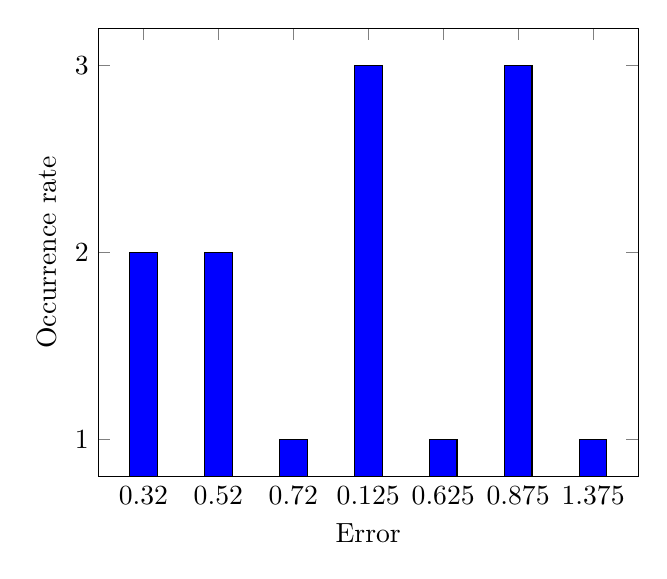
\begin{tikzpicture}
\begin{axis}[
	xlabel=Error,
	ylabel=Occurrence rate,
    symbolic x coords={0.32,0.52,0.72,0.125,0.625,0.875,1.375},
    ytick=data]
    \addplot[ybar,fill=blue] coordinates {
        (0.32, 2)
		(0.52, 2)
		(0.72, 1)
		(0.125, 3)
		(0.625, 1)
		(0.875, 3)
		(1.375, 1)
    };
\end{axis}
\end{tikzpicture}
\begin{center}
\caption{Errors of data points in found clusters}
\end{center}
\end{figure}



\chapter{CONCLUSION AND FUTURE WORK}
Abusing cloud resources is a prevalent threat toward cloud computing security. This is a threat which addresses mostly service providers than service consumers. Hence, it is vital for service providers to detect service misuses in their network. Detection of such misuses at the right time help to mitigate the threat with suitable countermeasures. The need for having effective monitoring systems is vital to empower security of the cloud. By making sure about security of the most inner entities of the cloud computing which are VMs, entire security of the cloud can be increased both for the service provider and the consumer. \\

In this document we presented a botcloud detection system. Our system detects members of botclouds that abuse cloud resources, among a crowd of VMs. As cloud's environment differ from conventional environments from various aspects, cloud's misuse detection systems should consider some considerations too. A cloud based detection system should be based on one of the cloud's core technologies. Our system is based on Virtualiazation techniques and takes advantage of data mining and virtual machine introspection techniques. Using mentioned technologies, based on some system level attributes and with regard to those attributes, our system groups VMs into two malicious and non-malicious. By identifying elements of botclouds which are grouped separately, the observable group under inspection gets smaller. As a result, further processes can take place on a smaller target group which consists malicious VMs. In this way, more accurate and reliable analysis can be done on a smaller group of targets which we know that they are malicious. In this regard, the possibility of wrong detection (false positive) in furtherer analysis would be eliminated. However correct grouping of machines in the fist place is very important in this regard. \\ 

We would like to further investigate the possibilities of applying classification techniques of data mining on the clustered data (malicious VMs cluster). In other word, we want to furtherer group the malicious VMs either with regard to other attributes. These attributes can be type of attacks they intend to have or type of malware which infected them. 

As user's data privacy is always an important matter, the matter of privacy arises here. Although VMI is a very powerful technique for security monitoring tools, at the same time it violates the user's privacy rules too. The information that are obtained by VMI technique, reveals some 
 Our future directions are: expanding the implementation by locating data collection modules in FVMs; testing the proposed solution in a cloud platform and providing methods to protect user's information privacy.\\



% insert references
%  � included unsrtf.bst provides finnish language version of unsrt
%    style, change below if needed
\bibliographystyle{unsrt}
\bibliography{thesisref}

%%%%%%%%%%%%%%%%%%%%%%%%%%%%%%%%%%%%%%%%%%%%%%%%%%%%%%%%%%%%%%%%%%%%%%%%%%%
%
% Almost there....
%
%%%%%%%%%%%%%%%%%%%%%%%%%%%%%%%%%%%%%%%%%%%%%%%%%%%%%%%%%%%%%%%%%%%%%%%%%%%

% make sure pagecount is correct even if references overflow to a new page
\pagebreak\addtocounter{page}{-1}
\eofpages
\appendices

% create your appendix chapters with command \appchapter{some name} instead
% of \chapter{some name} for the automagic page counting to work
%\input{file name of appchapter xxx}
%\input{file name of appchapter yyy}
%\input{file name of appchapter zzz}
%\input{and so on}

%%%%%%%%%%%%%%%%%%%%%%%%%%%%%%%%%%%%%%%%%%%%%%%%%%%%%%%%%%%%%%%%%%%%%%%%%%%
%
% main document ends here
%
%%%%%%%%%%%%%%%%%%%%%%%%%%%%%%%%%%%%%%%%%%%%%%%%%%%%%%%%%%%%%%%%%%%%%%%%%%%
\eofapppages
\end{document}


